\subsection{Overflow}
\label{subsec:overflow_description}
The overflow test case is an idealized domain designed to investigate the impact of topography on spurious mixing, and is similar to those found in \citet{Haidvogel_Beckmann99bk} and \citet[section 4]{Ilicak_ea12om}.  The domain is on a Cartesian plane of regularly spaced hexagons in the horizonal.  It is effectively two-dimensional, with dynamics occuring in the y-z plane, while the x-direction is four cells wide and periodic.  

This test case is useful for parameter studies to compare resolution, vertical mixing schemes, strength and types of horizontal mixing, partial bottom cells, and choice of vertical coordinate.  More advanced statistics, like the resting potential energy \citep{Ilicak_ea12om}, may be used to produce quantitative assessments of these comparisons.  The included test cases follow the parameters in \citet[section 4]{Ilicak_ea12om} and use zero explicit tracer mixing, Laplacian horizontal mixing of momentum with a viscosity of $10^3$ m$^2$/s, and constant vertical mixing of momentum with a viscosity of $10^{-4}$ m$^2$/s.  The equation of state is linear, and vertical coordinate is z-star \citep{Adcroft_Campin04om}.


\subsubsection{Provided Files}
\label{subsubsec:overflow_files}

\begin{itemize}
	\item grid.nc: \\
		This is the input grid file that includes initial conditions.  \\
		It can be visualized in the same way output files can to see the initial conditions.
	\item graph.info: \\
		This file is a graph of all of the cells in the mesh. \\
		It is used to decompose the mesh into partition files.
	\item graph.info.part.2: \\
		This is a partition file for use with a 2 processor run. \\
		The graph.info file has been decomposed into two blocks for this file.
	\item graph.info.part.4: \\
		This is a partition file for use with a 4 processor run. \\
		The graph.info file has been decomposed into four blocks for this file.
	\item graph.info.part.8: \\
		This is a partition file for use with a 8 processor run. \\
		The graph.info file has been decomposed into eight blocks for this file.
	\item namelist.input: \\
		This is the namelist file with all parameters for the run. \\
		It has a default setup which when run provides the results in the next section.
	\item visualize\_overflow.py: \\
		Python visualization script.  See Section \ref{sec:ocean_python}.
\end{itemize}

\subsubsection{Results}
\label{subsubsec:overflow_results}
Initially, a cold, dense volume of water is released at the top of a sill.  Within the course of an 18-hour simulation the cold water descends the steep mount and continues northward along the bottom.  The Coriolis parameter is set to zero so that rotational effects do not occur.  The speed of descent, or equivalently the time to reach the bottom, is a simple way to measure the amount of mixing that occurs as the plug of water descends.  In the two cases included with this release, the cold front reaches the bottom of the sill after eight hours for the high resolution case (1 km horizontal mesh, 100 layers), but after 16 hours for the low resolution case (10 km horizontal mesh, 40 layers).  Visualizations show that some ten-degree water remains after nine hours for the high-resolution case (Figure \ref{fig:overflow}), but has all mixed out for the low-resolution case (not shown).

The python script \verb|visualize_overflow.py| is included in the test case files to visualize cross-sections of cell-centered variables, like those shown in Figure \ref{fig:overflow}.  These plots may be created at the unix prompt with, for example,
\begin{verbatim}
python visualize_overflow.py -f output.nc -v temperature --min=10 --max=20 --time=9
\end{verbatim}
The python scripts are further described in Section \ref{sec:ocean_python}.

\begin{figure}[H!]
	\centering
	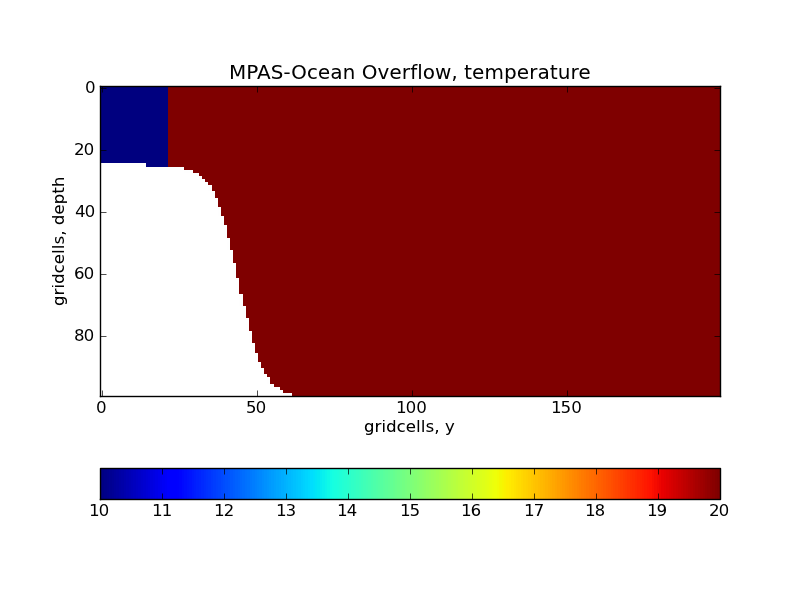
\includegraphics[scale=0.4]{ocean/figures/MPAS-O_overflow_temperature_0hrs.png}
	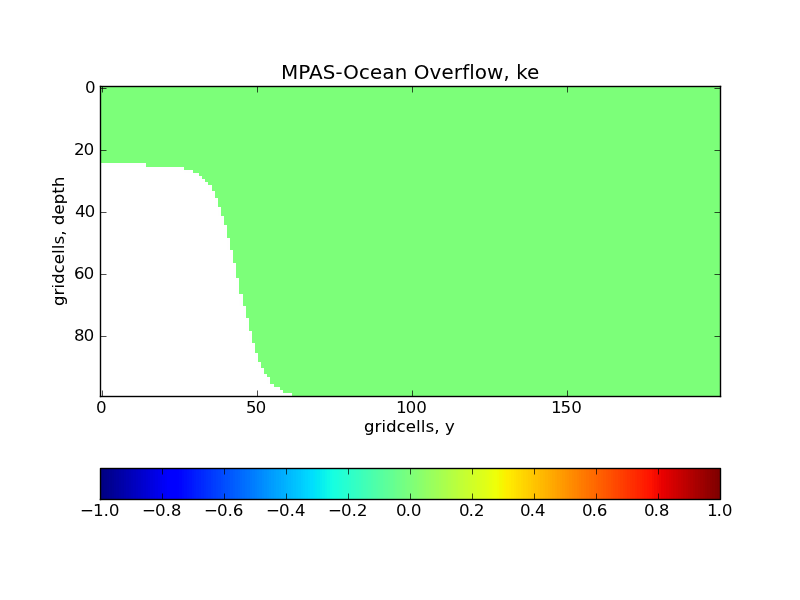
\includegraphics[scale=0.4]{ocean/figures/MPAS-O_overflow_ke_0hrs.png}\\
	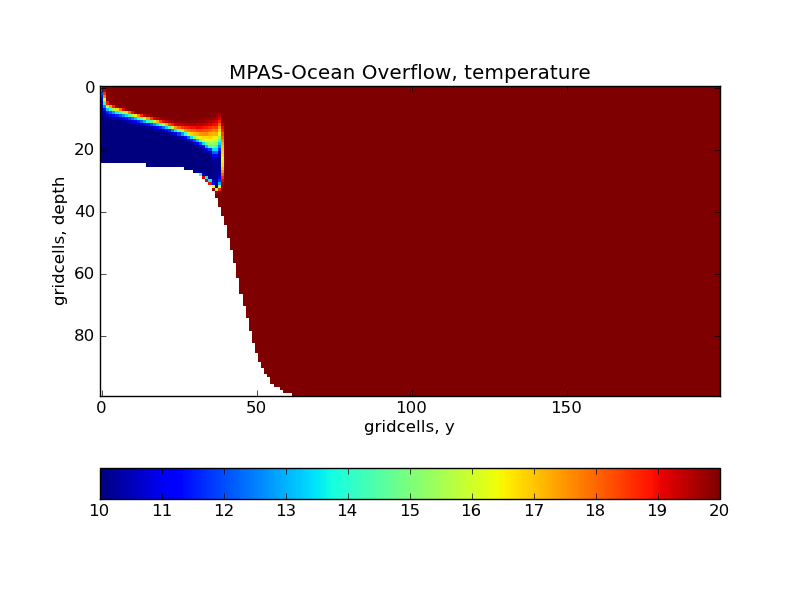
\includegraphics[scale=0.4]{ocean/figures/MPAS-O_overflow_temperature_3hrs.png}
	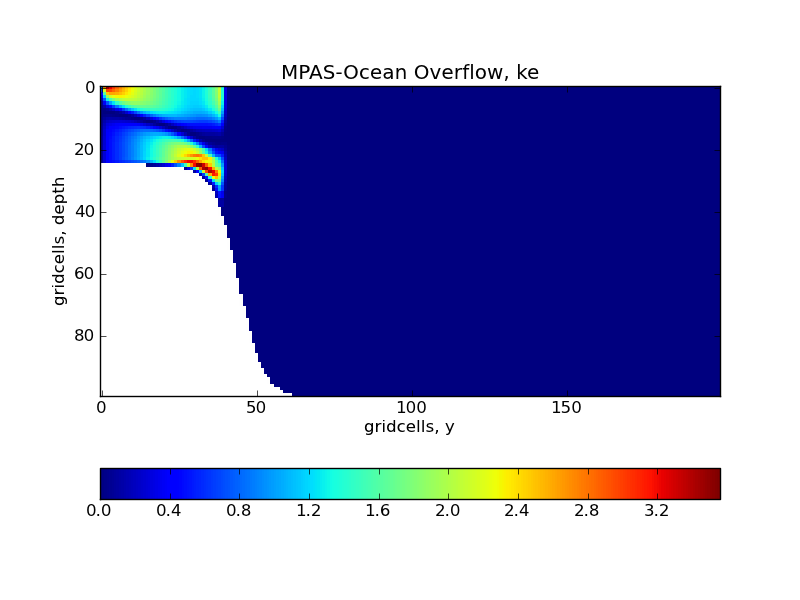
\includegraphics[scale=0.4]{ocean/figures/MPAS-O_overflow_ke_3hrs.png}\\
	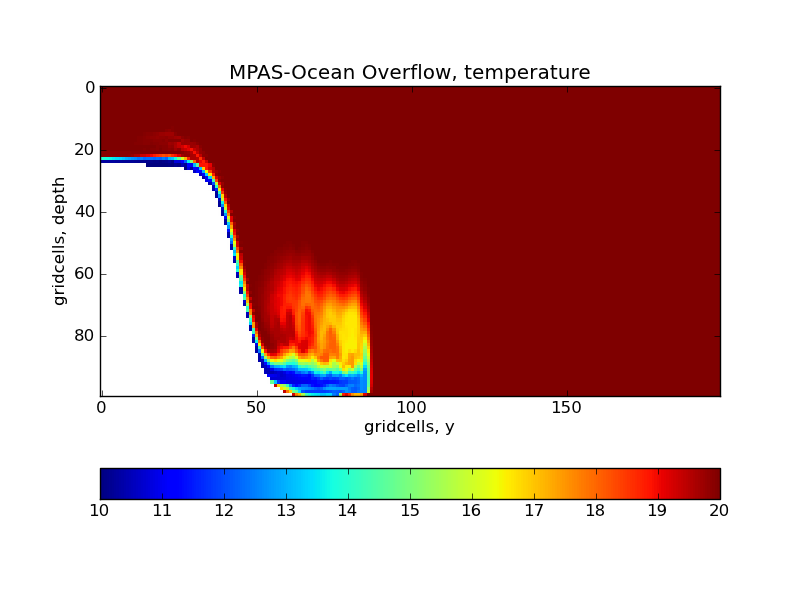
\includegraphics[scale=0.4]{ocean/figures/MPAS-O_overflow_temperature_9hrs.png}
	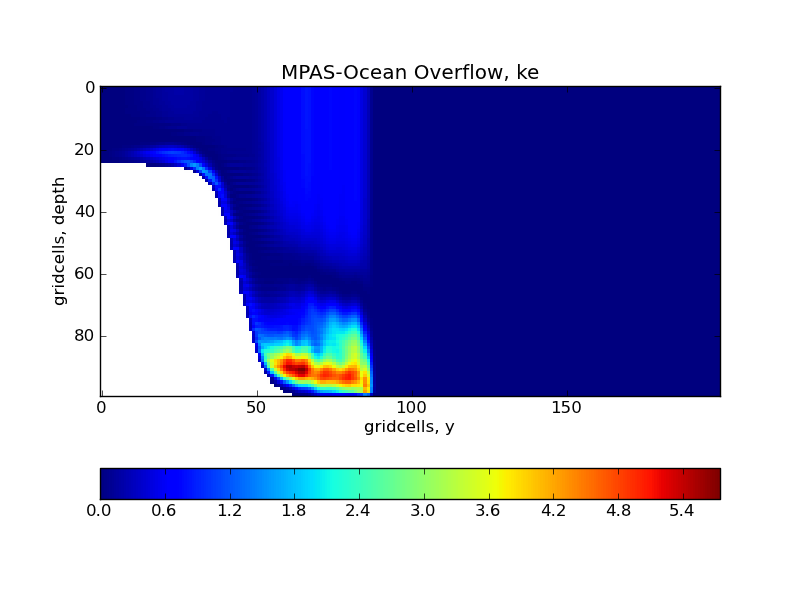
\includegraphics[scale=0.4]{ocean/figures/MPAS-O_overflow_ke_9hrs.png}
	\caption{Overflow test case results for the high resolution case (1 km horizontal grid-cells), showing vertical cross-sections of temperature (left) and kinetic energy (right).  Rows show initial condition (top), 3 hours (middle) and 9 hours (bottom).}
	\label{fig:overflow}
\end{figure}
